\begin{center}
    

\begin{tikzpicture}

    % Square in the middle
    \draw[thick] (2, 2) rectangle ++(4, 4);
    \draw[fill=magenta!50] (3, 3) rectangle ++(2, 2);

    % Label for the central area
    \draw[->, thick] (4.25, 3.5) -- ++(2, 2) node[right] {$G_c[e]$};

    \pgfmathsetseed{42}

    % Random red points inside the central area
    \foreach \i in {1,...,50} {
        \pgfmathsetmacro{\x}{3 + rnd*2}
        \pgfmathsetmacro{\y}{3 + rnd*2}
        \filldraw[fill=red] (\x,\y)  circle (2pt);
        % (3 + rand*2, 3 + rand*2)
    }

    % Random blue points outside the central area but inside the square
    \foreach \i in {1,...,15} {
        \pgfmathsetmacro{\x}{2 + rnd}
        \pgfmathsetmacro{\y}{2 + rnd*4}
        \filldraw[fill=blue] (\x,\y)  circle (2pt);
    }

    \foreach \i in {1,...,15} {
        \pgfmathsetmacro{\x}{2 + rnd*4}
        \pgfmathsetmacro{\y}{2 + rnd}
        \filldraw[fill=blue] (\x,\y)  circle (2pt);
    }

    \foreach \i in {1,...,15} {
        \pgfmathsetmacro{\x}{5 + rnd}
        \pgfmathsetmacro{\y}{2 + rnd*4}
        \filldraw[fill=blue] (\x,\y)  circle (2pt);
    }

    \foreach \i in {1,...,15} {
        \pgfmathsetmacro{\x}{2 + rnd*4}
        \pgfmathsetmacro{\y}{5 + rnd}
        \filldraw[fill=blue] (\x,\y)  circle (2pt);
    }

    \node[draw, fill=blue!20, text width=10cm, rounded corners] at (5, 0) {
            $ \xrightarrow{} $ One of the $(p+1)*(p+1)$ cells is considered $e$
            
            $ \xrightarrow{} $ For each connected component $H$ of $G_c[e]$, the subgraph of $G$ induced by $C[e]$ has a connected component dominating $H$
            };

\end{tikzpicture}

\end{center}